% Panel (a) of the hearing figure, split from fig-hearing.tex so the paper can present it as a
% subfigure (the (a)/(b) labels now come from LaTeX subcaptions, not baked into the image).
\documentclass[tikz,border=3pt]{standalone}
\usepackage{pgfplots}\pgfplotsset{compat=1.18}
\usepackage{times}
\begin{document}
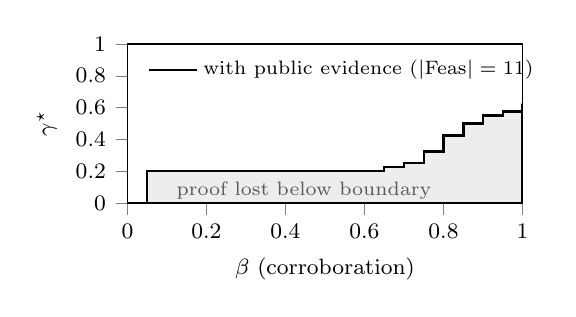
\begin{tikzpicture}
\begin{axis}[font=\footnotesize, width=6.6cm, height=3.6cm,
  xmin=0, xmax=1, xlabel={$\beta$ (corroboration)}, tick align=outside, tick pos=left,
  every axis plot/.append style={line width=0.9pt},
  ymin=0, ymax=1, ylabel={$\gamma^\star$},
  legend style={font=\scriptsize, at={(0.03,0.97)}, anchor=north west, draw=none, fill=none},
  legend cell align=left]
\addplot[const plot, black, fill=black, fill opacity=0.07, draw opacity=1]
  coordinates {(0.000,0.000) (0.050,0.200) (0.100,0.200) (0.150,0.200) (0.200,0.200) (0.250,0.200) (0.300,0.200) (0.350,0.200) (0.400,0.200) (0.450,0.200) (0.500,0.200) (0.550,0.200) (0.600,0.200) (0.650,0.225) (0.700,0.250) (0.750,0.325) (0.800,0.425) (0.850,0.500) (0.900,0.550) (0.950,0.575) (1.000,0.625)} \closedcycle;
\addlegendentry{with public evidence ($|\mathrm{Feas}|=11$)}
\node[font=\scriptsize, text=black!65, anchor=west] at (axis cs:0.10,0.08)
  {proof lost below boundary};
\end{axis}
\end{tikzpicture}
\end{document}
